% GNUPLOT: LaTeX picture with Postscript
\begingroup
  \makeatletter
  \providecommand\color[2][]{%
    \GenericError{(gnuplot) \space\space\space\@spaces}{%
      Package color not loaded in conjunction with
      terminal option `colourtext'%
    }{See the gnuplot documentation for explanation.%
    }{Either use 'blacktext' in gnuplot or load the package
      color.sty in LaTeX.}%
    \renewcommand\color[2][]{}%
  }%
  \providecommand\includegraphics[2][]{%
    \GenericError{(gnuplot) \space\space\space\@spaces}{%
      Package graphicx or graphics not loaded%
    }{See the gnuplot documentation for explanation.%
    }{The gnuplot epslatex terminal needs graphicx.sty or graphics.sty.}%
    \renewcommand\includegraphics[2][]{}%
  }%
  \providecommand\rotatebox[2]{#2}%
  \@ifundefined{ifGPcolor}{%
    \newif\ifGPcolor
    \GPcolortrue
  }{}%
  \@ifundefined{ifGPblacktext}{%
    \newif\ifGPblacktext
    \GPblacktexttrue
  }{}%
  % define a \g@addto@macro without @ in the name:
  \let\gplgaddtomacro\g@addto@macro
  % define empty templates for all commands taking text:
  \gdef\gplbacktext{}%
  \gdef\gplfronttext{}%
  \makeatother
  \ifGPblacktext
    % no textcolor at all
    \def\colorrgb#1{}%
    \def\colorgray#1{}%
  \else
    % gray or color?
    \ifGPcolor
      \def\colorrgb#1{\color[rgb]{#1}}%
      \def\colorgray#1{\color[gray]{#1}}%
      \expandafter\def\csname LTw\endcsname{\color{white}}%
      \expandafter\def\csname LTb\endcsname{\color{black}}%
      \expandafter\def\csname LTa\endcsname{\color{black}}%
      \expandafter\def\csname LT0\endcsname{\color[rgb]{1,0,0}}%
      \expandafter\def\csname LT1\endcsname{\color[rgb]{0,1,0}}%
      \expandafter\def\csname LT2\endcsname{\color[rgb]{0,0,1}}%
      \expandafter\def\csname LT3\endcsname{\color[rgb]{1,0,1}}%
      \expandafter\def\csname LT4\endcsname{\color[rgb]{0,1,1}}%
      \expandafter\def\csname LT5\endcsname{\color[rgb]{1,1,0}}%
      \expandafter\def\csname LT6\endcsname{\color[rgb]{0,0,0}}%
      \expandafter\def\csname LT7\endcsname{\color[rgb]{1,0.3,0}}%
      \expandafter\def\csname LT8\endcsname{\color[rgb]{0.5,0.5,0.5}}%
    \else
      % gray
      \def\colorrgb#1{\color{black}}%
      \def\colorgray#1{\color[gray]{#1}}%
      \expandafter\def\csname LTw\endcsname{\color{white}}%
      \expandafter\def\csname LTb\endcsname{\color{black}}%
      \expandafter\def\csname LTa\endcsname{\color{black}}%
      \expandafter\def\csname LT0\endcsname{\color{black}}%
      \expandafter\def\csname LT1\endcsname{\color{black}}%
      \expandafter\def\csname LT2\endcsname{\color{black}}%
      \expandafter\def\csname LT3\endcsname{\color{black}}%
      \expandafter\def\csname LT4\endcsname{\color{black}}%
      \expandafter\def\csname LT5\endcsname{\color{black}}%
      \expandafter\def\csname LT6\endcsname{\color{black}}%
      \expandafter\def\csname LT7\endcsname{\color{black}}%
      \expandafter\def\csname LT8\endcsname{\color{black}}%
    \fi
  \fi
    \setlength{\unitlength}{0.0500bp}%
    \ifx\gptboxheight\undefined%
      \newlength{\gptboxheight}%
      \newlength{\gptboxwidth}%
      \newsavebox{\gptboxtext}%
    \fi%
    \setlength{\fboxrule}{0.5pt}%
    \setlength{\fboxsep}{1pt}%
\begin{picture}(5760.00,2880.00)%
      \csname LTb\endcsname%%
      \put(2880,2694){\makebox(0,0){\strut{}Hagedorn (transmitted)wavepacket}}%
    \gplgaddtomacro\gplbacktext{%
      \colorrgb{0.50,0.50,0.50}%%
      \put(459,372){\makebox(0,0)[r]{\strut{}$0$}}%
      \colorrgb{0.50,0.50,0.50}%%
      \put(459,582){\makebox(0,0)[r]{\strut{}$0.1$}}%
      \colorrgb{0.50,0.50,0.50}%%
      \put(459,793){\makebox(0,0)[r]{\strut{}$0.2$}}%
      \colorrgb{0.50,0.50,0.50}%%
      \put(459,1003){\makebox(0,0)[r]{\strut{}$0.3$}}%
      \colorrgb{0.50,0.50,0.50}%%
      \put(459,1214){\makebox(0,0)[r]{\strut{}$0.4$}}%
      \colorrgb{0.50,0.50,0.50}%%
      \put(459,1424){\makebox(0,0)[r]{\strut{}$0.5$}}%
      \colorrgb{0.50,0.50,0.50}%%
      \put(459,1634){\makebox(0,0)[r]{\strut{}$0.6$}}%
      \colorrgb{0.50,0.50,0.50}%%
      \put(459,1845){\makebox(0,0)[r]{\strut{}$0.7$}}%
      \colorrgb{0.50,0.50,0.50}%%
      \put(459,2055){\makebox(0,0)[r]{\strut{}$0.8$}}%
      \colorrgb{0.50,0.50,0.50}%%
      \put(459,2266){\makebox(0,0)[r]{\strut{}$0.9$}}%
      \colorrgb{0.50,0.50,0.50}%%
      \put(459,2476){\makebox(0,0)[r]{\strut{}$1$}}%
      \colorrgb{0.50,0.50,0.50}%%
      \put(561,186){\makebox(0,0){\strut{}$2$}}%
      \colorrgb{0.50,0.50,0.50}%%
      \put(813,186){\makebox(0,0){\strut{}$2.5$}}%
      \colorrgb{0.50,0.50,0.50}%%
      \put(1064,186){\makebox(0,0){\strut{}$3$}}%
      \colorrgb{0.50,0.50,0.50}%%
      \put(1316,186){\makebox(0,0){\strut{}$3.5$}}%
      \colorrgb{0.50,0.50,0.50}%%
      \put(1567,186){\makebox(0,0){\strut{}$4$}}%
      \colorrgb{0.50,0.50,0.50}%%
      \put(1819,186){\makebox(0,0){\strut{}$4.5$}}%
      \colorrgb{0.50,0.50,0.50}%%
      \put(2070,186){\makebox(0,0){\strut{}$5$}}%
      \colorrgb{0.50,0.50,0.50}%%
      \put(2322,186){\makebox(0,0){\strut{}$5.5$}}%
      \colorrgb{0.50,0.50,0.50}%%
      \put(2573,186){\makebox(0,0){\strut{}$6$}}%
    }%
    \gplgaddtomacro\gplfronttext{%
      \csname LTb\endcsname%%
      \put(1785,2262){\makebox(0,0)[r]{\strut{}"~/NAQMD/src/Hagedorn/data/hag_wave".sprintf('%d%.3f', IX[i], DELTA[j])."_transmitted.txt"       using 1:(abs($4))}}%
    }%
    \gplgaddtomacro\gplbacktext{%
      \colorrgb{0.50,0.50,0.50}%%
      \put(3441,372){\makebox(0,0)[r]{\strut{}$0$}}%
      \colorrgb{0.50,0.50,0.50}%%
      \put(3441,673){\makebox(0,0)[r]{\strut{}$0.05$}}%
      \colorrgb{0.50,0.50,0.50}%%
      \put(3441,973){\makebox(0,0)[r]{\strut{}$0.1$}}%
      \colorrgb{0.50,0.50,0.50}%%
      \put(3441,1274){\makebox(0,0)[r]{\strut{}$0.15$}}%
      \colorrgb{0.50,0.50,0.50}%%
      \put(3441,1574){\makebox(0,0)[r]{\strut{}$0.2$}}%
      \colorrgb{0.50,0.50,0.50}%%
      \put(3441,1875){\makebox(0,0)[r]{\strut{}$0.25$}}%
      \colorrgb{0.50,0.50,0.50}%%
      \put(3441,2175){\makebox(0,0)[r]{\strut{}$0.3$}}%
      \colorrgb{0.50,0.50,0.50}%%
      \put(3441,2476){\makebox(0,0)[r]{\strut{}$0.35$}}%
      \colorrgb{0.50,0.50,0.50}%%
      \put(3543,186){\makebox(0,0){\strut{}$2$}}%
      \colorrgb{0.50,0.50,0.50}%%
      \put(3782,186){\makebox(0,0){\strut{}$2.5$}}%
      \colorrgb{0.50,0.50,0.50}%%
      \put(4021,186){\makebox(0,0){\strut{}$3$}}%
      \colorrgb{0.50,0.50,0.50}%%
      \put(4259,186){\makebox(0,0){\strut{}$3.5$}}%
      \colorrgb{0.50,0.50,0.50}%%
      \put(4498,186){\makebox(0,0){\strut{}$4$}}%
      \colorrgb{0.50,0.50,0.50}%%
      \put(4737,186){\makebox(0,0){\strut{}$4.5$}}%
      \colorrgb{0.50,0.50,0.50}%%
      \put(4976,186){\makebox(0,0){\strut{}$5$}}%
      \colorrgb{0.50,0.50,0.50}%%
      \put(5214,186){\makebox(0,0){\strut{}$5.5$}}%
      \colorrgb{0.50,0.50,0.50}%%
      \put(5453,186){\makebox(0,0){\strut{}$6$}}%
    }%
    \gplgaddtomacro\gplfronttext{%
      \csname LTb\endcsname%%
      \put(4665,2262){\makebox(0,0)[r]{\strut{}"~/NAQMD/src/Hagedorn/data/hag_wave".sprintf('%d%.3f', IX[i], DELTA[j])."_transmitted.txt"       using 1:(abs($4))}}%
    }%
    \gplbacktext
    \put(0,0){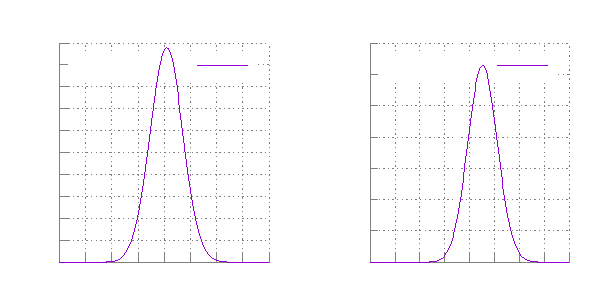
\includegraphics{/home/s1992054/NAQMD/src/Hagedorn/plots/hagedorngaussian}}%
    \gplfronttext
  \end{picture}%
\endgroup
